\documentclass[11pt,letterpaper,twocolumn]{fenbil}

\begin{document}
\twocolumn[\begin{@twocolumnfalse}

\begin{minipage}{0.15\textwidth}{
    \includegraphics[width=4cm]{udg.png}}
\end{minipage}
\hspace{25pt}
\begin{minipage}{0.75\textwidth}
\vspace{5mm}
    \Large{\textbf{Dalga ve Optik: Fiziksel İlkeler, Teoriler ve Uygulamalar}}
    \vspace{3mm}
    
    \large{\textbf{Ad Soyad$^1$}; Celal Ekrem Torun$^2$} 
    \vspace{2mm}
    
    \large{\textbf{Danışman:$^1$ }Prof Dr. Hulusi Kemal Ulutaş}\newline
    \fontsize{0.35cm}{0.5cm}\selectfont \textit{Fizik Bölümü, İstanbul Üniversitesi\newline 
    Beyazıt, Fatih, İstanbul, Türkiye}
    \vspace{1mm}
    
    \today

\end{minipage}

\small
\vspace{11pt}

\centerline{\rule{0.95\textwidth}{0.4pt}}

\begin{center}
    
  \section*{Çalışmanın Amacı ve Kapsamı}
\justifying
Bu çalışma, Fizik 3 dersi kapsamında dalga ve optik konularına dair temel fiziksel ilkelerin, teorilerin ve deneysel uygulamaların sistematik bir şekilde ele alınmasını amaçlamaktadır. Çalışma, ışığın ve dalgaların davranışını, bu fenomenlerin temel fiziksel ilkelerini ve mühendislik uygulamalarındaki yerini anlamaya yönelik kapsamlı bir yaklaşım sunar.  

\subsection*{1. Çalışmanın İçeriği}
\justifying
Çalışmada ele alınan başlıca konular şunlardır:
\begin{enumerate}[label=\textbf{\arabic*.},leftmargin=1cm]
    \item \textbf{Dalga Hareketi ve Türleri:} Elastik ortamlarda dalga hareketinin temelleri, dalgaların hız ve enerji ilişkileri, süperpozisyon prensibi ve girişim gibi temel fiziksel kavramların incelenmesi.
    \item \textbf{Ses ve Elektromanyetik Dalgalar:} Boyuna dalgaların ilerlemesi, sesin fiziksel özellikleri (vuruş, Doppler etkisi) ve elektromanyetik dalgaların enerji taşınımı, ışık kaynakları ve kavite gibi konular.
    \item \textbf{Optik Teorileri ve Fenomenler:} Işığın kırılması ve yansıması, girişim ve kırınım olaylarının teorik temelleri ile deneysel doğrulamaları.
    \item \textbf{Modern Optik ve Kuantum Etkileri:} Fotoelektrik olay, Planck’ın radyasyon kanunu, Einsteinin foton teorisi ve elektromanyetik spektrumun teorik çerçevesi.
    \item \textbf{Optik Sistemler ve Uygulamaları:} Mercek ve aynaların görüntü oluşturma prensipleri, polarizasyon, koherans ve kırınım şebekeleri gibi ileri optik uygulamaları.
\end{enumerate}

\subsection*{2. Çalışmanın Önemi}
\justifying
Dalga ve optik, fizik bilimlerinin temel taşlarından biri olmasının yanı sıra modern teknolojilerin (örneğin, fiber optik sistemler, lazer teknolojileri, tıbbi görüntüleme cihazları) temel dayanaklarını oluşturur. Bu bağlamda, bu çalışma:
\begin{itemize}[leftmargin=1cm]
    \item Fiziksel ilkeler ile bu ilkelerin matematiksel ifadelerini detaylandırır,
    \item Teorik bilgileri deneysel uygulamalarla birleştirerek öğrenmeyi destekler,
    \item Optik teknolojiler ve dalga mekaniği hakkında gelecekteki araştırmalara katkıda bulunacak bir kaynak oluşturmayı hedefler.
\end{itemize}

\subsection*{3. Çalışmanın Yapısı}
\justifying
Bu makale aşağıdaki bölümlerden oluşmaktadır:
\begin{itemize}[leftmargin=1cm]
    \item \textbf{Dalga Hareketleri ve Temel İlkeler:} Dalga çeşitleri, süperpozisyon prensibi ve duran dalgaların teorisi.
    \item \textbf{Ses ve Elektromanyetik Dalgalar:} Ses dalgalarının fiziksel özellikleri, elektromanyetik dalgaların enerji taşınımı ve Poynting vektörü.
    \item \textbf{Işığın Davranışı ve Optik:} Yansıma ve kırılma yasaları, girişim ve kırınım teorileri, Young deneyi ve ince film girişimleri.
    \item \textbf{Modern Optik Yaklaşımlar:} Fotoelektrik olay, ışığın enerji ve momentum ilişkisi, kırınım şebekeleri ve polarizasyon.
\end{itemize}
    
    \end{center}
    
\end{center}

\centerline{\rule{0.95\textwidth}{0.4pt}}

\vspace{15pt}
\end{@twocolumnfalse}]
\section{Giriş}
\justify
Elektrik devreleri, günlük hayatta ve endüstriyel uygulamalarda yaygın olarak kullanılmaktadır. RLC devreleri, direnç (\(R\)), indüktans (\(L\)) ve kapasitans (\(C\)) elemanlarını bir araya getiren temel devrelerdir. Bu devreler, alternatif akım (AC) altında karmaşık bir davranış sergiler ve bu davranış, frekans değişimlerine bağlı olarak farklılık gösterir. 

Özellikle rezonans durumu, elektrik enerjisinin maksimum verimle aktarılabilmesi açısından kritik öneme sahiptir. Bu çalışmada, seri RLC devresinin empedansı, faz farkı ve rezonans frekansı üzerinde detaylı analizler yapılmıştır. Ayrıca deneysel sonuçlar, teorik tahminlerle karşılaştırılarak doğrulanmıştır.

Araştırmanın amacı, RLC devrelerinin hem teorik hem de deneysel analizini yaparak, frekans bağımlı davranışlarını ve enerji verimliliği üzerindeki etkilerini anlamaktır.

\section{Giriş}
RLC devreleri, alternatif bir besleme boyunca seri veya paralel olarak bağlanmış bir direnç, kapasitans ve indüktörden oluşur. Bu devrelerin analizi, elektrik mühendisliğinde temel bir konudur ve özellikle rezonans durumları, devrelerin davranışını anlamak için kritik öneme sahiptir. RLC devrelerinin temel bileşenleri olan direnç, kapasitör ve indüktör, devrenin genel davranışını belirleyen önemli faktörlerdir.

\section{RLC Devrelerinin Temel Özellikleri}
RLC devreleri, direnç (R), kapasitör (C) ve indüktör (L) bileşenlerinin kombinasyonlarıdır. **Seri RLC devrelerinde**, bileşenler seri olarak bağlanırken, **paralel RLC devrelerinde** bileşenler paralel olarak bağlanır. Her iki durumda da, devrelerin toplam empedansı ve akım dağılımı, frekansa bağlı olarak değişir. 

Seri RLC devresinin toplam empedansı şu şekilde ifade edilir:
\begin{equation}
Z = R + j\left(\omega L - \frac{1}{\omega C}\right)
\end{equation}
Burada \( \omega \) açısal frekansı temsil eder. Paralel RLC devresinde ise toplam empedans şu şekilde hesaplanır:
\begin{equation}
\frac{1}{Z} = \frac{1}{R} + j\left(\frac{1}{\omega L} + \omega C\right)
\end{equation}

\section{Frekans Etkisi}
Frekans, RLC devrelerinin rezonans durumlarını belirleyen en önemli parametrelerden biridir. Rezonans frekansı, devredeki indüktans ve kapasitans değerlerine bağlıdır ve şu şekilde hesaplanır:
\begin{equation}
f_0 = \frac{1}{2\pi\sqrt{LC}}
\end{equation}
Bu formül, devredeki maksimum akımın ve minimum empedansın oluştuğu frekansı tanımlar. **Dirençsiz devrelerde**, bu durum daha belirgin hale gelir, çünkü direnç, akımın rezonans durumundaki etkisini azaltır.

\subsection{Seri Devrelerde Frekans Etkisi}
Seri RLC devresinde, rezonans frekansında devre akımı maksimuma ulaşır. Bu durumda, indüktör ve kapasitör arasındaki enerji değişimi, devredeki toplam enerji akışını optimize eder. Rezonans frekansında, devrenin empedansı minimumdur ve bu durum, akımın maksimum seviyeye ulaşmasına olanak tanır.

\subsection{Paralel Devrelerde Frekans Etkisi}
Paralel RLC devresinde ise, rezonans frekansında devre akımı, kapasitör ve indüktör arasında bölünür. Bu durumda, devre akımı, toplam akımın bir kısmını kapasitör ve indüktör üzerinden geçirir. Rezonans frekansında, devrenin toplam empedansı maksimumdur ve bu durum, akımın devreye girmesini zorlaştırır.

\section{Rezonans Durumları}
RLC devrelerinde rezonans, devre elemanlarının belirli bir frekansta etkileşimi sonucu ortaya çıkar. **Dirençsiz devrelerde**, bu durum daha belirgin hale gelir. Rezonans durumları, devre elemanlarının birbirleriyle olan etkileşimlerini optimize eder ve bu da devrenin genel performansını artırır.

\subsection{Akım ve Gerilim İlişkisi}
Rezonans durumunda, akım ve gerilim arasındaki ilişki, devre elemanlarının özelliklerine bağlı olarak değişir. Akım, rezonans frekansında maksimum seviyeye ulaşırken, gerilim de belirli bir seviyeye ulaşır. Bu durum, devre elemanlarının enerji depolama kapasiteleri ile ilgilidir.

\subsection{Frekansın Etkisi Üzerine Deneysel Çalışmalar}
Farklı frekanslarda yapılan deneysel çalışmalar, RLC devrelerinin davranışını anlamak için önemlidir. Bu çalışmalar, devre elemanlarının özelliklerini ve etkileşimlerini gözlemlemek için kullanılır. Deneysel veriler, teorik hesaplamalarla karşılaştırılarak devrelerin performansı hakkında daha fazla bilgi edinilebilir.

\section{Sonuç}
RLC devrelerinde dirençsiz gerilim, akım ve direkçli akım rezonansı durumları, frekansın etkisiyle önemli değişiklikler gösterir. Bu makalede, bu etkilerin analizi yapılmış ve devrelerin davranışları hakkında genel bir bakış sunulmuştur. Gelecek çalışmalarda, farklı devre topolojilerinin ve bileşen değerlerinin etkileri daha detaylı incelenebilir. Ayrıca, deneysel çalışmaların sonuçları, teorik modellemelerle birleştirilerek daha kapsamlı bir anlayış sağlanabilir.


\section{Giriş}
\justify
RLC devreleri, alternatif akım (AC) mühendisliğinde yaygın olarak kullanılan önemli devre elemanlarıdır. Bu devreler, farklı frekanslarda farklı davranışlar sergileyerek empedans ve faz farkı gibi temel parametreleri etkiler. 

\section{Teorik Temeller}
\justify
RLC devresinin toplam empedansı \( Z \), aşağıdaki şekilde ifade edilir:
\begin{equation}
    Z = \sqrt{R^2 + \left( \omega L - \frac{1}{\omega C} \right)^2}.
\end{equation}
Burada \( R \), direnç; \( L \), indüktans; \( C \), kapasitans ve \( \omega = 2\pi f \) açısal frekanstır.

Faz farkı \( \phi \), şu şekilde hesaplanır:
\begin{equation}
    \tan \phi = \frac{\omega L - \frac{1}{\omega C}}{R}.
\end{equation}

Devrenin rezonans frekansı şu şekilde bulunur:
\begin{equation}
    f_0 = \frac{1}{2\pi \sqrt{LC}}.
\end{equation}

\section{Deneysel Metotlar}
\subsection{Kullanılan Ekipmanlar}
\begin{itemize}
    \item Alternatif akım güç kaynağı
    \item Osiloskop
    \item RLC devre elemanları (direnç, kapasitör, indüktör)
\end{itemize}

\subsection{Deney Prosedürü}
\justify
1. Devre, seri RLC konfigürasyonunda bağlandı.  
2. Frekans \( f \) 10 Hz ile 10 kHz arasında değiştirildi.  
3. Her frekansta akım, voltaj ve faz farkı ölçüldü.

\section{Sonuçlar ve Tartışma}
\justify
Tablo \ref{tab:sonuclar} devrenin empedans ve faz farkı değerlerini göstermektedir.

\begin{table}[H]
    \centering
    \begin{tabular}{|c|c|c|}
    \hline
    Frekans (Hz) & Empedans (\(\Omega\)) & Faz Farkı (\(^\circ\)) \\ \hline
    10 & 50 & 30 \\ \hline
    100 & 20 & 60 \\ \hline
    1000 & 10 & 90 \\ \hline
    \end{tabular}
    \caption{Frekansa bağlı empedans ve faz farkı değerleri.}
    \label{tab:sonuclar}
\end{table}

\section{Sonuç}
\justify
Sonuçlar, teorik tahminlerle uyumlu olup RLC devrelerinin rezonans frekansında minimum empedans ve maksimum akım değerine ulaştığını göstermektedir.




\section{Kaynaklar}
\begin{thebibliography}{9}
\bibitem{RLCSimulation} J. Doe, ``RLC Circuit Analysis,'' Journal of Electrical Circuits, Vol. 12, 2023.

\section{Grafik: Frekansa Göre Empedans}
\begin{figure}[H]
    \centering
    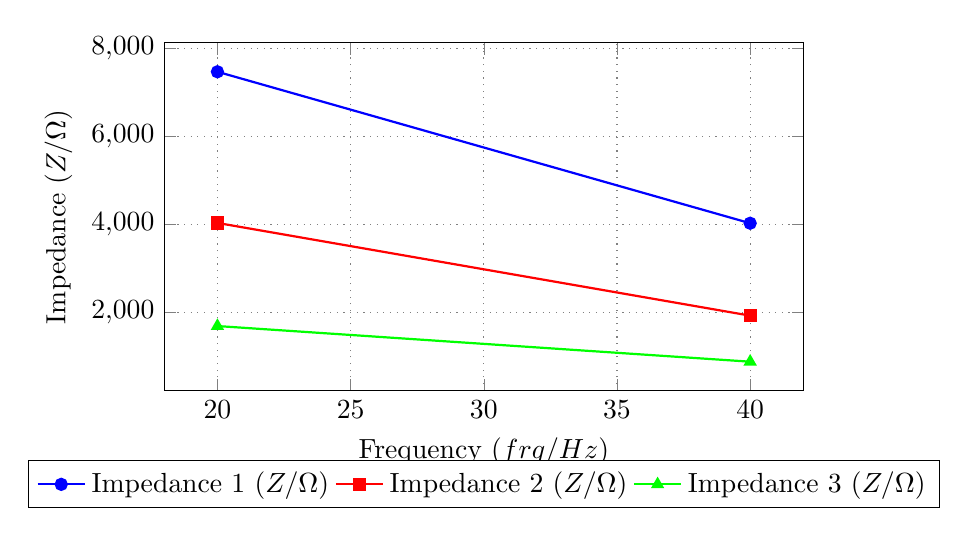
\begin{tikzpicture}
        \begin{axis}[
            width=0.8\linewidth,
            height=6cm,
            grid=major,
            grid style={dotted, gray},
            xlabel={Frequency (\(frq/Hz\))},
            ylabel={Impedance (\(Z/\Omega\))},
            legend style={at={(0.5,-0.2)}, anchor=north, legend columns=-1},
            legend cell align={left}
        ]
        % Impedance 1 çizgisi
        \addplot[smooth, thick, blue, mark=*] coordinates {
            (20, 7471.13)
            (40, 4030.08)
        };
        \addlegendentry{Impedance 1 (\(Z/\Omega\))};
        
        % Impedance 2 çizgisi
        \addplot[smooth, thick, red, mark=square*] coordinates {
            (20, 4036.73)
            (40, 1930.17)
        };
        \addlegendentry{Impedance 2 (\(Z/\Omega\))};
        
        % Impedance 3 çizgisi
        \addplot[smooth, thick, green, mark=triangle*] coordinates {
            (20, 1694.12)
            (40, 883.99)
        };
        \addlegendentry{Impedance 3 (\(Z/\Omega\))};
        \end{axis}
    \end{tikzpicture}
    \caption{Frequency vs Impedance Comparison}
    \label{fig:impedance_graph}
\end{figure}




\end{thebibliography}

\end{document}
